\begin{figure}[t]
\centering
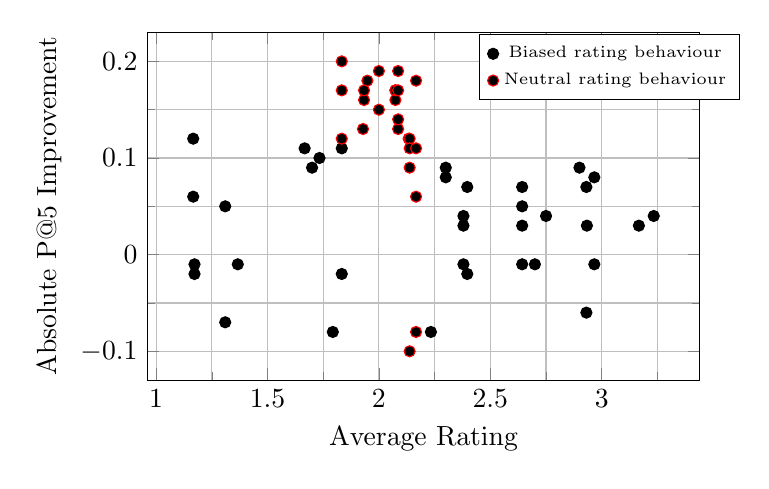
\begin{tikzpicture}
\begin{axis}[%
ylabel=Absolute P@5 Improvement ,
xlabel=Average Rating,
scatter/classes={%
    a={mark=*,draw=black},
    b={mark=*,draw=red}
    },
width= 8.6cm, %\textwidth,
height=6cm, %5cm,
grid = both,
legend columns=2,
grid = both,
minor tick num=1,
legend columns=1, 
legend style={
        at={(0.6,0.90)},
        anchor=west,
        font=\fontsize{6}{7}\selectfont,
        /tikz/column 2/.style={
            column sep=5pt,
        },
    },
% scatter/classes={
% 	a={mark=square*,draw=b},%
% 	b={mark=triangle*,draw=g},%
% },
]
\addplot[scatter,only marks,%
    scatter src=explicit symbolic]%
table[meta=label] {
x     y      label
1.1666666667	0.06	a
1.1666666667	0.12	a
1.1724137931	-0.01	a
1.1724137931	-0.02	a
1.3103448276	0.05	a
1.3103448276	-0.07	a
1.3666666667	-0.01	a
1.6666666667	0.11	a
1.7	0.09	a
1.7333333333	0.1	a
1.7931034483	-0.08	a
1.8333333333	0.11	a
1.8333333333	-0.02	a
1.8333333333	0.12	b
1.8333333333	0.17	b
1.8333333333	0.2	b
1.9285714286	0.13	b
1.9333333333	0.16	b
1.9333333333	0.17	b
1.9482758621	0.18	b
2	0.19	b
2	0.15	b
2.0740740741	0.17	b
2.0740740741	0.16	b
2.0740740741	0.17	b
2.0862068966	0.13	b
2.0862068966	0.19	b
2.0862068966	0.17	b
2.0862068966	0.14	b
2.1333333333	0.12	b
2.1379310345	0.12	b
2.1379310345	-0.1	b
2.1379310345	0.11	b
2.1379310345	0.09	b
2.1666666667	-0.08	b
2.1666666667	0.06	b
2.1666666667	0.11	b
2.1666666667	0.18	b
2.2333333333	-0.08	a
2.3	0.09	a
2.3	0.08	a
2.3793103448	0.03	a
2.3793103448	-0.01	a
2.3793103448	0.04	a
2.3965517241	0.07	a
2.3965517241	-0.02	a
2.6428571429	-0.01	a
2.6428571429	0.03	a
2.6428571429	0.05	a
2.6428571429	0.07	a
2.7	-0.01	a
2.75	0.04	a
2.9	0.09	a
2.9310344828	0.07	a
2.9310344828	-0.06	a
2.9333333333	0.03	a
2.9666666667	0.08	a
2.9666666667	-0.01	a
3.1666666667	0.03	a
3.2333333333	0.04	a
    };

\legend{Biased rating behaviour, Neutral rating behaviour}
\end{axis}
\end{tikzpicture}
\caption{\label{fig:gprates}Improvement of the performance of contextual suggestion by help of group profiles for users with different rating behavior.}
    \end{figure}